\documentclass[notes,tikz,minted]{agony}

\declaretheorem[name=Warm-Up Exercise,refname={WE,WEs},style=thmquoteresult,parent=chapter]{warmup}
\declaretheoremstyle[
	headfont=\bfseries\color{OliveGreen},
  notefont=\mdseries,
	bodyfont=\normalfont,
	mdframed={style=mdquote,linecolor=ForestGreen,backgroundcolor=ForestGreen!5},
]{thmquotegreen}
\declaretheorem[name=Recommended Problem,refname={RP,RPs},style=thmquotegreen,parent=chapter]{recommended}
\declaretheorem[name=Challenge,refname={C,Cs},style=thmquotered,parent=chapter]{challenge}

\title{MATH 135 Fall 2020: Extra Practice}
\author{James Ah Yong and contributors}
\begin{document}
\thispagestyle{firstpage}

\chapter*{MATH 135 Fall 2020:\\{\huge Extra Practice}}

\begin{mdframed}[style=mdround,linecolor=red,backgroundcolor=CarnationPink!5]
  This document was entirely written by then-first year Double Degrees.
  \textbf{\color{Red}{Nothing here is official. There are no guarantees that content is remotely close to correct.}}
  If you find a mistake, please either \href{https://agony.retrocraft.ca/#contact}{let me know}
  or make a \href{https://github.com/RetroCraft/problems/pulls}{pull request} fixing it.

  \textbf{\color{Red}{Try the problems first}} before looking at solutions.
  You won't learn by reading someone else's work.
\end{mdframed}

\begin{multicols*}{2}
  % Print ToC without ToC title
  \makeatletter
  \@starttoc{toc}
  \makeatother
\end{multicols*}

\section{Linear programs}

\lecture{May 2}
\begin{example}
  Suppose we are selling apples and bananas at a stand.
  Apples sell for \$2 per kilogram, and bananas sell for \$1.5 per kilogram.
  Our stand holds up to 75 kilograms of fruits.
  Also, there are only 4 square metres of shelf space.
  Each kilogram of apples/bananas takes up roughly 0.08/0.05 square metres of shelf space, respectively.
  How much of each fruit should we stock to maximize the total sales?
\end{example}
\begin{sol}
  Let $x_1$, $x_2$ be weight of apples, bananas (kg).
  Define objective function $\max\ 2x_1 + 1.5x_2$.
  Add constraints $x_1 + x_2 \leq 75$ for weight, $0.08x_1 + 0.05x_2 \leq 4$ for shelf space, and $x_1, x_2 \geq 0$ for common sense.

  Summarize as a \term*{linear program}:
  \begin{equation*}
    \begin{aligned}
      \max\                      &  & \multicolumn{2}{l}{$2x_1 + 1.5x_2$}           \\
      \text{subject to (s.t.)}\  &  & x_1 + x_2                           & \leq 75 \\
                                 &  & 0.08x_1 + 0.05x_2                   & \leq 4  \\
                                 &  & x_1, x_2                            & \geq 0
    \end{aligned}
  \end{equation*}

  Trial and error:
  \begin{itemize}[nosep]
    \item $(x_1, x_2) = (30, 20)$ satisfies constraints (\term*{feasible}) with \term*{objective value} 90
    \item $(x_1, x_2) = (31, 20)$ feasible with objective value 92
    \item $(x_1, x_2) = (50, 0)$ feasible with objective value 100
    \item $(x_1, x_2) = (8\frac13, 66\frac23)$ feasible with objective value 116$\frac23$
          (claim without proof that this is \term*{optimal})
  \end{itemize}

  N.B.: we take domain to be $\R$ since we can take fractional parts of a kilogram of fruit

  Plot feasible solutions:
  \begin{center}
    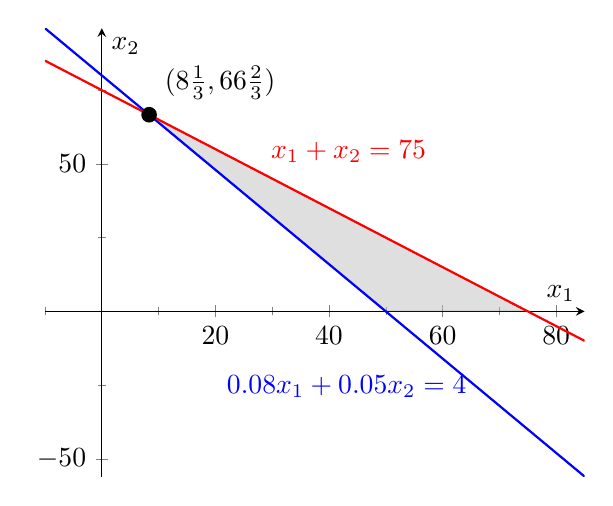
\begin{tikzpicture}
      \begin{axis}[
          axis lines=middle,
          xlabel=$x_1$,
          ylabel=$x_2$,
          minor tick num=1,
        ]
        \addplot[fill=gray!50, opacity=0.5] coordinates {(25/3,200/3) (50,0) (75,0)} -- cycle;
        \addplot[domain=-10:85, blue, thick] {(4-0.08*x)/0.05} node[left, pos=0.8] {$0.08x_1 + 0.05x_2 = 4$};
        \addplot[domain=-10:85, red, thick] {75-x} node[above right, pos=0.4] {$x_1 + x_2 = 75$};
        \node[fill=black, circle, inner sep=2pt, label={above right:$(8\frac13,66\frac23)$}] at (25/3,200/3) {};
      \end{axis}
    \end{tikzpicture}
  \end{center}
  Bound by convex region defined by axes, $x_1 + x_2 = 23$,
  and $0.08x_1 + 0.05x_2 = 4$ to give optimal solution at vertex
\end{sol}

\paragraph{Course overview}
\begin{itemize}[nosep]
  \item Formulation/modelling: create mathematical programs from problems
  \item Solving linear programs: use simplex method to optimize
  \item Geometric interpretation: conceptualize linear programs and simplex method
  \item Integer programs: linear programs defined over $\Z$
  \item Nonlinear programs: convex functions
\end{itemize}

\begin{defn}[optimization problem]
  Given a set of \term{feasible points} $A \subseteq \R^n$ and $f : A \to \R$,
  find some $x \in A$ that minimizes or maximizes the \term{objective value} $f(x)$.

  Composed of \term{decision variables} $\vb x \in \R^n$,
  the \term{objective function} $\max f(\vb x)$ or $\min f(\vb x)$,
  and some \term{constraints} of the form $g_i(\vb x) \leq b_i$
\end{defn}

\begin{defn}[affine function]
  Function of the form $f(\vb x) = \vb a^T \vb x + b = a_1x_1 + \dotsb + a_nx_n + b$ for constants $\vb a$ and $b$
\end{defn}

\begin{defn}[linear function]
  Affine function with $b=0$
\end{defn}

\begin{defn}[linear program]
  An optimization problem with affine objective function $f(\vb x)$ and finitely many linear constraint functions $g_i(x) \geq b_i$ (or $\leq b_i$ or $= b_i$) with constant $\vb b$.

  N.B.: constraints cannot be strict inequalities
\end{defn}

\section{LP Formulation}

\begin{example}
  A company makes 4 types of products, each requiring time on two different machines and two types of labour. The amount of machine time and labour needed to produce one unit of each product along with its sale price are summarized in the following table.
  \begin{center}
    \begin{tabular}{c|ccccc}
      Product & Machine 1 & Machine 2 & Skilled labour & Unskilled labour & Unit sale price \\ \hline
      1       & 11        & 4         & 8              & 7                & 300             \\
      2       & 7         & 6         & 5              & 8                & 260             \\
      3       & 6         & 5         & 5              & 7                & 220             \\
      4       & 5         & 4         & 6              & 4                & 180             \\
    \end{tabular}
  \end{center}
  Each month, the company can use up to 700 hours on machine 1, and 500 hours on machine 2, with no cost. The company can hire up to 600 hours of skilled labour at \$8 per hour, and up to 650 hours of unskilled labour at \$6 per hour. How should the company operate to maximize their monthly profit?
\end{example}
\begin{sol}
  Let $\vb x \in \R^4$ be number of units of products, $y_s$ and $y_u$ be hours of labour hired

  Let the objective function be $\max \enspace 300 x_1 + 260 x_2 + 220 x_3 + 180 x_4 - 8y_s - 6y_u$ (unit sale revenue net of labour costs)

  Let the constraints be $11x_1 + 7x_2 + 6x_3 + 5x_4 \leq 700$ (machine 1), $4x_1 + 6x_2 + 5x_3 + 4x_4 \leq 500$ (machine 2), $8x_1 + 5x_2 + 5x_3 + 6x_4 = y_s$, $7x_1 + 8x_2 + 7x_3 + 4x_4 = y_u$ (defining $y_s$ and $y_u$), $y_s \leq 600$, $y_u \leq 650$ (labour), and $x_1, x_2, x_3, x_4, y_s, y_u \geq 0$ (non-negativity)
\end{sol}

\lecture{May 4}
\begin{example}
  A certain company provides heading oil for the local commnity. They have historical data that helps them predict demand for heating oil in the next four months: 5000, 8000, 9000, 6000 (litres/month)

  At the beginning of each month, they can purchase oil from the supplier at the current market rate. The projected rates are given: 0.75, 0.72, 0.92, 0.90 (\$/litre)

  There is a storage tank that holds up to 4000 litres of oil, and at the start of month 1, it contains 2000 litres. How should the company buy the required oil to minimize the total money spent?
\end{example}
\begin{sol}
  Let $x_i$ be the amount of oil purchased in the $i$th month, and $y_i$ be the amount of oil in the storage tank at the start of month $i$.

  Then, we want to minimize $0.75x_1 + 0.72x_2 + 0.92x_3 + 0.9x_4$.

  The storage tank constrains us by $y_i \leq 4000$ and the problem gives $y_1 = 2000$.

  Non-negativity gives $x_i, y_i \geq 0$.

  For each demand $d_i$, we have $x_i + y_i = d_i + y_{i+1}$.

  Then, we can write:
  \begin{lp}{\min}{0.75x_1 + 0.72x_2 + 0.92x_3 + 0.9x_4}
     &  & y_1, y_2, y_3, y_4              & \leq 4000    \\
     &  & y_1                             & = 2000       \\
     &  & x_1 + y_1                       & = 5000 + y_2 \\
     &  & x_2 + y_2                       & = 8000 + y_3 \\
     &  & x_3 + y_3                       & = 9000 + y_4 \\
     &  & x_4 + y_4                       & = 6000       \\
     &  & x_1,x_2,x_3,x_4,y_1,y_2,y_3,y_4 & \geq 0
  \end{lp}
\end{sol}

\begin{example}
  Instead of minimizing the total money spent, suppose we do not have much money to spend each month, and we want to reduce the maximum amount spent in a month.
\end{example}
\begin{sol}
  Let $M = \max \{0.75x_1, 0.72x_2, 0.92x_3, 0.9x_4\}$.

  Since $M$ is not linear, we cannot simply put $\min M$ in an LP.

  Instead, define $m$ with constraints $m \geq 0.75x_1$, $m \geq 0.72x_2$, $m \geq 0.92x_3$, $m \geq 0.9x_4$.

  Since we are doing $\min m$, we are guaranteed that the optimal solution will give $m = M$ (if $m$ is not $M$, we can make $m$ smaller).
\end{sol}

\begin{example}
  Given a set of data points $\{(x_i, y_i) : i = 1,\dotsc,n\}$ on the plane. Find a line $y = ax + b$ that ``best fits'' this set of data points.
\end{example}
\begin{sol}
  Define ``best fit'' as minimizing total vertical distance between points and the line.

  That is, we must minimize $\sum \abs{ax_i + b - y_i}$, but that is not affine.

  Define instead the errors $e_i$ associated with the point $i$.

  We want to constrain $e_i = \abs{ax_i + b - y_i}$, which we can do with $e_i \geq ax_i + b - y_i$ and $e_i \geq y_i - ax_i - b$ since $\abs{x} = \max\{x, -x\}$.

  Then, we can use $\min \sum e_i$ as above to get the final LP:
  \begin{align*}
    \min \        & \sum e_i                \\
    \text{s.t.}\  & e_i \geq ax_i + b - y_i \\
                  & e_i \geq y_i - ax_i - b
  \end{align*}
  \textbf{N.B.:} since $e_i$, $e_j$ do not share constraints when $i \neq j$, $\min \sum e_i$ is equivalent to $\min e_1, \dotsc, \min e_n$.
\end{sol}

\begin{xca}
  Modify this to find the best fit parabola. Is this an LP?
\end{xca}
\begin{sol}
  Yes, since considering the error function $ax_i^2 + bx_i + c - y_i$ is still linear with respect to the variables for optimization $a$, $b$, and $c$.
\end{sol}

\section{Formulating IPs}

\lecture{May 9}
\begin{example}
  Consider the job application process where a company has 3 positions available, and there are 4 applicants for these jobs. For each applicant and position, the company assigns a number indicating how well the applicant is suited for the position. The goal is to hire a different applicant for each position to maximize the total suitability.

  \[
    M = \begin{pNiceMatrix}[first-row,first-col]
                                            & \Block{1-4}{\text{Candidates}} &   &   &   \\
      \Block{3-1}{\rotate \text{Positions}} & 3                              & 5 & 2 & 4 \\
                                            & 3                              & 1 & 4 & 3 \\
                                            & 1                              & 4 & 2 & 3
    \end{pNiceMatrix}
  \]
\end{example}
\begin{sol}
  Want: For each position, who gets that position

  Define: Create binary variable $x_{ij}$ for each position $i$ and candidates $j$. Let $x_{ij} = 1$ if position $i$ given to candidate $j$, and $0$ otherwise

  Objective function: $\max \sum\sum M_{ij}x_{ij}$

  Constraints: $\sum_{j} x_{ij} = 1$ for each $i$ (each position filled by exactly one candidate), and $\sum_i x_{ij} \leq 1$ for each $j$  (each candidate takes at most one position), $x_{ij} \geq 0$, $x_{ij} \leq 1$, $x_{ij} \in \Z$ (integrality)
  \begin{align*}\max\ & \sum_{i=0}^3\sum_{j=0}^4 M_{ij}x_{ij} \\ \text{s.t.}\ & \sum_{j=0}^4 x_{ij} = 1 & i = 1,\dotsc,3 \\ &\sum_{i=0}^3 x_{ij} \leq 1 & j = 1,\dotsc,4 \\ & 0 \leq x_{ij} \leq 1, x_{ij} \in \Z\end{align*}
\end{sol}

\begin{notation}
  We define $x \in \{0,1\}$ to mean the constraints $0 \leq x \leq 1$ and $x \in \Z$
\end{notation}

\begin{example}[Knapsack problem]
  There are 4 types of items that you can put into your backpack. You can take any integer number of units of any item. However, you can only carry a maximum of 40 pounds. Each unit of item you take is also worth a certain amount of money. The goal is to maximize the total value of the items you carry.
  \begin{center}
    \begin{tabular}{r|cccc}
      Item         & A  & B  & C  & D  \\ \hline
      Weight (lbs) & 1  & 7  & 3  & 2  \\
      Value (\$)   & 10 & 50 & 20 & 15 \\
    \end{tabular}
  \end{center}
\end{example}
\begin{sol}
  Let $x_i$, $i = A,B,C,D$ be the number of units of $i$ packed

  Objective function: $\max 10x_A + 50x_B + 20x_C + 15x_D$

  Constraints: $x_A + 7x_B + 3x_C + 2x_D \leq 40$ (weight limit), $x_i \geq 0$, $x_i \in \Z$ (integrality)

  \[
    \begin{aligned}
      \max\         &  & 10x_A + 50x_B + 20x_C + 15x_D           \\
      \text{s.t.}\  &  & x_A + 7x_B + 3x_C + 2x_D      & \leq 40 \\
                    &  & x_A,x_B,x_C,x_D               & \geq 0  \\
                    &  & x_A,x_B,x_C,x_D               & \in \Z
    \end{aligned}
  \]
\end{sol}

\begin{example}
  Suppose we are allowed to take A only if we take at least one unit of B.
\end{example}
\begin{sol}
  Want: if $x_B = 0$, then we must have $x_A = 0$. If $x_B \geq 1$, no restriction on $A$.

  Equivalently, add the constraint $x_A \leq x_B \max x_A = 40x_B$. When $x_B = 0$, the RHS goes to $0$ and constrains $x_A = 0$. Otherwise, since $x_B \geq 1$, $40x_B \geq 40$ which is the maximum value of $x_A$, so there are effectively no constraints on $x_A$.
\end{sol}

\begin{example}
  Suppose we want the following conditions to hold:
  \begin{enumerate}[1.,nosep]
    \item We carry at least 5 units of items A and/or B; or
    \item We carry at least 7 units of items C and/or D.
  \end{enumerate}
\end{example}
\begin{sol}
  Define a binary variable $y$. Want: $y = \begin{cases*}1&condition 1 is true\\0&condition 2 is true\end{cases*}$

  If $y = 1$, then $x_A + x_B \geq 5$; if $y = 0$, no restrictions on $x_A$, $x_B$. We can implement this by adding the constraint $x_A + x_B \geq 5y$, since $y = 0$ will send the RHS to $0$

  If $y = 0$, then $x_C + x_D \geq 7$; if $y = 1$, no restrictions on $x_C$, $x_D$. Similarly implement with $x_C + x_D \geq 7(1-y)$, since $y=1$ will send the RHS to $0$

  Notice that setting $y$ does not force the other condition \emph{not} to hold, i.e., this implements an inclusive or.

  In summary: $x_A + x_B \geq 5y$, $x_C + x_D \geq 7(1-y)$, and $y \in \{0,1\}$

  \textbf{N.B.:} When feeding these constraints into an algorithm, ensure that the constraints are truly linear, i.e., move variables to one side. For example, $x_A + x_B - 5y \geq 0$
\end{sol}

\begin{xca}
  Implement an exclusive or of these two conditions
\end{xca}

\begin{example}
  Suppose that the value of item A is \$10 for the first 5 units, but any more units beyond that has value \$5.
\end{example}
\begin{sol}
  Separate $x_A$ into two variables $x_{A1}$ for first five units and $x_{A2}$ for remainder.
  Then, we have $x_A=x_{A1}+x_{A2}$ and change the objective function to $10x_{A1} + 5x_{A2} + 50x_B + 20x_C + 15x_C$.

  We can create a constraint to force $x_{A2}$ only to go up when $x_{A1}$ is 5 with $x_{A2} \leq (x_{A1} - 4)\max x_{A2}$ which will work in tandem with the non-negativity constraint. This is not actually necessary since the maximum will always fill $x_{A1}$ before $x_{A2}$ because it is worth more (i.e. trading one $x_{A2}$ for $x_{A1}$ will increase the objective function by 5)

  In summary: change the objective function and add the constraints $x_A = x_{A1} + x_{A2}$, $x_{A1} \leq 5$, $x_{A1},x_{A2} \geq 0$, $x_{A1}, x_{A2} \in \Z$
\end{sol}

\lecture{May 11}
\begin{notation}[vector notation]
  Write $\mathbb{1} := (1,\dotsc,1)^T$ and $x \leq y$ if $x_i \leq y_i$ for all $i$.
\end{notation}

\begin{defn}[graph]
  $G = (V, E)$ consists of a set of objects $V$ (\term{vertices}) and a set of unordered pairs of vertices $E$ (\term{edges}).

  We restrict graphs by disallowing empty graphs, redundant edges, directed edges, or self-connections.
\end{defn}

\begin{example}\label{ex:graph}
  $G = (V, E)$ by $V = \{1,2,3,4\}$, $E=\{12,23,34,41,24\}$
  \begin{center}
    \tikz\graph{{1,4}--{2,3}; 1--4; 2--3; 2--4};
  \end{center}
\end{example}

\begin{defn}[incidence relation]
  For an edge $e=uv$, $e$ is incident to $u$ and $v$.
  $\delta(v)$ is the set of all edges incident to $v$.

  The \term{incidence matrix} $B \in \{0,1\}^{\abs{V}\times\abs{E}}$
  has rows indexed by $V$, columns by $E$, and $B_{ve} = 1$
  when $e \in \delta(v)$ and $0$ otherwise.
\end{defn}
\begin{example}
  For \cref{ex:graph}, $B = \begin{pNiceMatrix}[first-row,first-col]
        & e_1 & e_2 & e_3 & e_4 & e_5 \\
      1 & 1   & 0   & 0   & 1   & 0   \\
      2 & 1   & 1   & 0   & 0   & 1   \\
      3 & 0   & 1   & 1   & 0   & 0   \\
      4 & 0   & 0   & 1   & 1   & 1
    \end{pNiceMatrix}$.
\end{example}
\begin{remark}
  Each column has exactly two ones, so $B\mathbb{1} = 2\mathbb{1}$.
\end{remark}

\begin{defn}[matching]
  $M \subseteq E$ where each vertex is incident with exactly zero or one edge in $M$ (i.e., $\abs{M \cap \delta(v)} \leq 1$ for all $v \in V$)
\end{defn}
\begin{example}
  For \cref{ex:graph}, $\{e_1, e_3\}$ and $\{e_5\}$ are matchings but $\{e_1, e_5\}$ is not since $2$ is incident to both edges
\end{example}

\begin{example}[maximum-weight matching]
  Given graph $G = (V, E)$ and weights $w_e$ for each $e \in E$. Find a matching in $G$ with the maximum edge weight, i.e., maximize $\sum_{e \in M} w_e$.
\end{example}
\begin{sol}
  Define a vector $x \in \{0,1\}^{\abs{E}}$ by $x_e = 1$ if $e \in M$ and $0$ otherwise.
  Then, the objective function is $\max w^T x$.
  To ensure each node appears only once, add constraints $\sum_{e \in \delta(v)} x_e \leq 1$ for each $v \in V$. This is equivalent to taking the incidence matrix $A$ and saying $Ax \leq \mathbb{1}$
  This gives us the integer program
  \begin{align*}
    \max\         & w^T x                         \\
    \text{s.t.}\  & Ax \leq \mathbb{1}            \\
                  & x_e \in \{0,1\} \quad e \in E
  \end{align*}
\end{sol}

\begin{defn}[$v_1$,$v_k$-path]
  Sequence of edges $v_1v_2, v_2v_3, \dotsc, v_{k-1}v_k$ such that $v_1,\dotsc,v_k$ are distinct
\end{defn}
\begin{example}\label{ex:path}
  Consider graph $(\{s,t,a,b,c,d\}, \{sa,sc,ab,ac,bd,bt,cb,cd,dt\})$.
  \begin{center}
    \begin{tikzpicture}
      \graph[math nodes]{s--{a--b,c--d}--t; a--c; b--d; c--b};
    \end{tikzpicture}
  \end{center}  
  Then, $sa,ab,bt$ and $sc,cb,bd,dt$ are $s$,$t$-paths but $sa,ab,bc,cd,cb,bt$ is not since $b$ is visited twice.
\end{example}

\lecture{May 16}

\begin{problem}[shortest path]
  Given graph $G = (V, E)$, vertices $s$ and $t$, and positive weights $w_e$ for each $e \in E$. Find an $s$,$t$-path $P$ with the minimum edge weight, i.e., minimize $\sum_{e \in P} w_e$.
\end{problem}

Define a vector $x \in \{0,1\}^{\abs{E}}$ by $x_e = 1$ if $e \in P$ and $0$ otherwise.

The objective function is $\min w^T x$.

Need to constrain $x$ into a path: use cuts.

\begin{defn}[cut]
  The \term*{cut induced by vertices $W$} is the set $\delta(W)$ of all edges with exactly one endpoint in $W$.
  Formally, $\delta(W) = \{uv \in E : u \in W, v \not\in W\}$.

  An \term{$s,t$-cut} $\delta(W)$ has $s \in W$ and $t \not\in W$.
\end{defn}
\begin{example}
  In \cref{ex:path}, $W=\{s,a,b\}$ induces the cut $\delta(W) = \{sc,ac,bc,bd,bt\}$
  \begin{center}
    \begin{tikzpicture}
      \graph[math nodes,simple]{s--{a--b,c--d}--t; s--[red]c; a--[red]c; b--[red]d; b--[red]c; b--[red]t};
    \end{tikzpicture}
  \end{center}
\end{example}

\begin{prop}
  Notice that the edges in an $s,t$-cut separate $s$ from $t$, so an $s,t$-path must use at least one edge from every $s,t$-cut (formal proof in graph theory course)
\end{prop}

We get a constraint $\sum_{e \in \delta(W)} x_e \geq 1$ for all $s,t$-cuts $\delta(W)$ (that is, for all $W \subset V$ with $s \in W$ and $t\not\in W$)

\begin{prop}
  If a set of edges intersects every $s,t$-cut, then it contains an $s,t$-path
\end{prop}

Minimizing the edge weights will ensure that the extraneous edges are optimized away and the $s,t$-path remains so long as the edge weights are all positive.

This gives us a final IP of
\begin{align*}
  \min\         & w^T x                                                               \\
  \text{s.t.}\  & \sum_{e \in \delta(W)} x_e \geq 1 & \text{$\delta(W)$ an $s,t$-cut} \\
                & x_e \geq 0, x_e \in \Z            & e \in E
\end{align*}

\section{Formulating NLPs}

\begin{defn}[non-linear program]
  A program of the general form $\min f(x)$ subject to $g_i(x) \leq 0$ for some arbitrary functions $f : \R^n \to \R$, $g_i : \R^n \to \R$ with no restrictions
\end{defn}
\begin{example}
  Among all the points $x$ that satisfy $Ax \leq b$, find one that is closest to the target point $\bar x$
\end{example}
\begin{sol}
  We can take the norm and minimize $\norm{x - \bar x} = \sqrt{\sum(x_i-\bar x_i)^2}$.
  This gives us the non-linear program $\min \norm{x - \bar x}, \text{s.t.\ } Ax \leq b$.
\end{sol}

\lecture{May 18}
Since the definition for NLP has no constraints on $f$ and $g_i$, a LP is an NLP.

The integrality constraint makes IPs not NLPs.
To get around this, use a periodic function like $\sin \theta = 0$ which permits values $\theta = k\pi$ for integer $k$, so $x \in \Z \Harr \sin x\pi  = 0$.
Using this makes IPs into NLPs.

If we can solve NLPs, we can also solve LPs and IPs.

\section{LP outcomes}

An algorithm that solves LPs should produce:
\begin{itemize}[nosep]
  \item The optimal solution (or that no solution exists)
  \item Certificate of correctness that reduces complexity of verification
\end{itemize}

\begin{defn}[infeasibility]
  No feasible solutions exist.
\end{defn}

\begin{example}
  $\max x$ s.t. $x \leq 2$ and $x \geq 3$. Obviously, no $x$ exists.
\end{example}

\begin{example}
  $\max{(3,1,-7,4)x}$ s.t. $\mqty(-5&4&3&-1\\2&1&-5&3\\-1&-3&1&-2)x = \mqty(3\\-2\\1)$ and $x \geq \mathbb{0}$.

  Taking $-2R_1 - 3R_2 - 4R_3$, we get $8x_1+x_2+5x_3+x_4 = -4$ but each entry in $x$ must be non-negative, so this is impossible.

  Formally, we can let $y = (-2,-3,-4)^T$, then multiply on the left by $y^T$ to give us the same equation as $(8,1,5,1)x = -4$.

  Then, $y$ is the \term{certificate of infeasibility}.
\end{example}

\begin{prop}
  The system $Ax = b$, $x \geq \mathbb{0}$ is infeasible if there exists a vector $y$ such that $y^T A \geq \mathbb{0}$ but $y^T b < 0$
\end{prop}
\begin{prf}
  Suppose the system is feasible with $x$ as the feasible solution. Then, $Ax = b$ and $x \geq \mathbb{0}$. However, $y^T A x \geq 0$ and $y^T b < 0$. Contradiction.
\end{prf}

The converse is also true. Proof will come later as Farkas' Lemma.

\begin{defn}[unboundedness]
  Infinitely better feasible solutions exist.

  Formally, a max (resp. min) LP is \term*{unbounded} if there exists a series of feasible solutions $x(t)$ with the objective value of $x(t)$ approaching $+\infty$ (resp. $-\infty$) as $t \to \infty$.
\end{defn}
\begin{example}
  $\max x$ s.t. $x \geq 1$: there is no best solution (cf. strict inequalities)
\end{example}
\begin{example}
  $\max{} (-1,2,-3,4)x$ s.t. $\mqty(3&0&2&-5\\-2&3&-4&4)x=\mqty(4\\1)$ and $x \geq \mathbb 0$.

  Consider $\bar x = (3,1,0,1)^T$ and $d = (0,4,5,2)^T$. Define $x(t) = \bar x + td$ and consider $t$ from $0 \to \infty$.
  We must show feasibility and unboundedness.

  Obviously, $x(t) \geq \mathbb 0$ since $\bar x, d \geq \mathbb 0$ and $t \geq 0$.

  Notice $Ax(t) = A\bar x + tAd = (4,1)^T + t(0,0)^T = b$. That is, $\bar x$ solves $Ax = b$ and $d$ lies in the kernel of $A$.

  The objective value $c^T x(t) = c^T(\bar x + td) = c^T\bar x + tc^T d = 3 + t$ clearly goes to $+\infty$ as $t \to \infty$.

  Then, $(\bar x, d)$ is a certificate of unboundedness for the LP.
\end{example}

\begin{prop}
  The LP $\max \{c^T x : Ax=b, x \geq \mathbb 0\}$ is unbounded if there exist vectors $\bar x$ and $d$ such that $\bar x, d \geq \mathbb 0$, $Ad = \mathbb 0$, $c^T d > 0$.
\end{prop}

\chapter{Logical Analysis of Mathematical Statements}

\section{Warm-Up Exercises}
\begin{warmup}
  Let $A$, $B$ and $C$ be statement variables.
  Determine the truth table of $(A \land B) \implies \lnot C$.
\end{warmup}
\begin{sol}
  ~

  \begin{center}
    \begin{tabular}{C|C|C|C|C|C}
      A & B & C & A \land B & \lnot C & (A \land B) \implies \lnot C \\ \hline
      T & T & T & T         & F       & F                            \\
      T & T & F & T         & T       & T                            \\
      T & F & T & F         & F       & T                            \\
      T & F & F & F         & T       & T                            \\
      F & T & T & F         & F       & T                            \\
      F & T & F & F         & T       & T                            \\
      F & F & T & F         & F       & T                            \\
      F & F & F & F         & T       & T                            \\
    \end{tabular}
  \end{center}
\end{sol}

\begin{warmup}
  State the contrapositive and the converse of the following implication: If Jane is a doctor, then she went to medical school.
\end{warmup}
\begin{sol}
  \emph{Converse}: If Jane went to medical school, then she is a doctor.
  \emph{Contrapositive}: If Jane did not go to medical school, then she is not a doctor.
\end{sol}

\section{Recommended Problems}
\begin{recommended}
  For each of the following statements, identify the four parts of the quantified statement (quantifier, variables, domain, and open sentence).
  Next, express the statement in symbolic form using as few words as possible and then write down the negation of the statement
  (when possible, without using any negative words such as “not” or the $\lnot$ symbol, but negative math symbols like $\neq$ are okay).
  Finally determine if the original statement is true or false. No justification is needed.
  \begin{enumerate}
    \item For all real numbers $x$ and $y$, $x \neq y$ implies that $x^2+y^2 > 0$.
    \item For every even integer $a$ and odd integer $b$, a rational number $c$ can always be found such that $a<c<b$ or $b<c<a$.
  \end{enumerate}
\end{recommended}
\begin{sol}
  \begin{enumerate}
    \item \[ \forall x\in\R, \forall y\in\R, x \neq y \implies x^2+y^2>0 \]
          Quantifier: universal;
          variable: $x$;
          domain: $\R$;
          open sentence: $x \neq y \Rarr x^2+y^2>0$.
          Negation: $\exists x\in\R, \exists y\in\R, x \neq y \land x^2+y^2\leq0$.
          The statement is \emph{true}.
    \item \[
            \forall a\in\Z, \forall b\in\Z, \exists c\in\Q,
            \left(\frac{a}{2}\in\Z \land \frac{b-1}{2}\in\Z\right) \implies (a<c<b \lor b<c<a)
          \]
          Quantifier: universal/existential;
          variables: $a$, $b$, $c$;
          domain: $\Z$, $\Q$;
          open sentence: $(\frac{a}{2}\in\Z \land \frac{b-1}{2}\in\Z) \Rarr (a<c<b \lor b<c<a)$.
          Negation:
          \[
            \exists a\in\Z, \exists b\in\Z, \forall c\in\Q,
            \qty(\frac{a}{2}\in\Z \land \frac{b-1}{2}\in\Z) \land
            \qty((c \leq a \lor c \geq b) \land (c \leq b \lor c \geq a))
          \]
          The statement is \emph{true}.
          \qedhere
  \end{enumerate}
\end{sol}

\begin{recommended}
  Let $A$ and $B$ be statement variables.
  Prove that $(\lnot A) \lor B$ is logically equivalent to $\lnot(A \land \lnot B)$.
\end{recommended}
\begin{prf}
  Apply De Morgan's law: $(\lnot A) \lor B \equiv \lnot(A \land \lnot B)$.
\end{prf}


\begin{recommended}
  Let $A$ and $B$ be statement variables.
  Determine whether $A \implies B$ is logically equivalent to $(\lnot A) \lor B$.
\end{recommended}
\begin{prf}
  $A \implies B$ is defined as $\lnot(A \land \lnot B)$.
  This is easily verifiable by noticing that an implication is only false when the hypothesis is true but the conclusion is false.
  Expand using De Morgan's law: $\lnot(A \land \lnot B) \equiv (\lnot A \lor B)$.
\end{prf}


\begin{recommended}
  Assume that it has been established that the following implication is true:
  \begin{center}
    If I don't see my advisor today, then I will see her tomorrow.
  \end{center}
  For each of the sentences below, determine if it is true or false. No justification is needed.
  If you can't determine the truth value of the sentence, explain why.
  \begin{enumerate}
    \item I don't meet my advisor both today and tomorrow. (This is arguably an ambiguous English sentence. Answer the problem using both interpretations.)
    \item I meet my advisor both today and tomorrow.
    \item I meet my advisor either today or tomorrow (but not on both days).
  \end{enumerate}
\end{recommended}
\begin{sol}
  \begin{enumerate}
    \item For the case of not today and not tomorrow, the statement is contradictory.
          For the case of today or tomorrow, exclusive, see (c).
    \item Not contradictory, but the truth value is indeterminate because we do not know about meeting ``today''.
    \item Not contradictory, but the truth value is indeterminate because we do not know about meeting ``today''.
          \qedhere
  \end{enumerate}
\end{sol}

\begin{recommended}
  Let $A$, $B$ and $C$ be statement variables.
  Prove the following logical equivalence using a chain of logical equivalences as in Chapter 2.3 of the notes.
  \[
    (A \land C) \lor (B \land C) \equiv \lnot((A \lor B) \implies \lnot C)
  \]
\end{recommended}
\begin{prf}
  Begin by considering the implication on the right-hand side.
  Recall the definition of an implication $X \implies Y \equiv \lnot X \lor Y$.
  Apply this and simplify:
  \begin{align*}
    \lnot((A \lor B) \implies \lnot C) & \equiv \lnot(\lnot (A \lor B) \lor \lnot C)                                           \\
                                       & \equiv \lnot(\lnot (A \lor B)) \land \lnot(\lnot C) & \text{De Morgan's law}          \\
                                       & \equiv (A \lor B) \land C                           & \text{Double negation}          \\
                                       & \equiv (A \land C) \lor (B \land C)                 & \text{Distributive conjunction}
  \end{align*}
  Hence, the left side is logically equivalent to the right side, so the equivalency holds.
\end{prf}

\begin{recommended}
  Four friends: Alex, Ben, Gina and Dana are having a discussion about going to the movies.
  Ben says that he will go to the movies if Alex goes as well.
  Gina says that if Ben goes to the movies, then she will join.
  Dana says that she will go to the movies if Gina does.
  That afternoon, exactly two of the four friends watch a movie at the theatre.
  Deduce which two people went to the movies.
\end{recommended}
\begin{prf}
  For each friend, let $A$, $B$, $G$, and $D$ be if they go to the movies, respectively.
  We can write our statements as implications: $A \implies B$, $B \implies G$, and $G \implies D$.
  By the transitivity of the implication, $A \implies G$, $A \implies D$, and $B \implies D$.
  Recall that only two of $A$, $B$, $G$, and $D$ are allowed to be simultaneously true.
  If $A$ is true, then all of $B$, $G$, and $D$ are true, which is a contradiction.
  Therefore, $A$ is false.
  If $B$ is true, then both $G$ and $D$ are true, which is a contradiction.
  Therefore, $B$ is false.
  This leaves $G$ (which implies $D$) and $D$ to be true, which satisfies our exclusivity condition.
  Therefore, Gina and Dana atttended the movies.
\end{prf}

\begin{recommended}
  Consider the following statement.
  \begin{center}
    For all $x\in\R$, if $x^6 + 3x^4 - 3x < 0$, then $0 < x < 1$
  \end{center}
  \begin{enumerate}
    \item Rewrite the given statement in symbolic form.
    \item State the hypothesis of the implication within the given statement.
    \item State the conclusion of the implication within the given statement.
    \item State the converse of the implication within the given statement.
    \item State the contrapositive of the implication within the given statement.
    \item State the negation of the given statement without using the word ``not''
          or the $\lnot$ symbol (but symbols such as $\neq$, $\nmid$, etc.\ are fine).
  \end{enumerate}
\end{recommended}
\begin{sol}
  \begin{enumerate}
    \item $\forall x\in\R, x^6 + 3x^4 - 3x < 0 \implies 0 < x < 1$
    \item $x^6 + 3x^4 - 3x < 0$
    \item $0 < x < 1$
    \item $0 < x < 1 \implies x^6 + 3x^4 - 3x < 0$
    \item $x \leq 0 \lor x \geq 1 \implies x^6 + 3x^4 - 3x \geq 0$
    \item $\exists x\in\R, x^6 + 3x^4 - 3x < 0 \land (x \leq 0 \lor x \geq 1)$
          \qedhere
  \end{enumerate}
\end{sol}

\include{extra-practice/03proofs}
\include{extra-practice/04induction}
\chapter{Sets}

\section{Warm-Up Exercises}

\begin{warmup}
  Let $\U=\{1,2,3,4,5,6,7,8,9\}$, $A=\{2,4,6,9\}$, and $B=\{4,5,6,7\}$.
\end{warmup}
\begin{enumerate}[(a)]
  \item Calculate the following:
        \begin{enumerate}[i.]
          \item $A \cup B = \{2,4,5,6,7,9\}$
          \item $A \cap B = \{4,6\}$
          \item $\overline{A} = \U - A = \{1,3,5,7,8\}$
          \item $\overline{B} = \U - B = \{1,2,3,8,9\}$
          \item $A-B = \{2,9\}$
          \item $B-A = \{5,7\}$
        \end{enumerate}
  \item Are $A$ and $B$ disjoint? \emph{No, since 4 is in both sets.}
  \item Give a set $C$ such that $C \subseteq B$. \emph{Let $C=B$.}
  \item Give a set $D$ such that $D \subsetneq A$. \emph{Let $D=\{2\}$.}
\end{enumerate}

\begin{warmup}
  Suppose $S$ and $T$ are two sets.
  Prove that if $S \cap T = S$, then $S \subseteq T$.
  Is the converse true?
\end{warmup}
\begin{proof}
  Let $S$ and $T$ be arbitrary sets such that their intersection is $S$.
  We must show that any element of $S$ is an element of $T$.

  Consider an element $s$ in $S$.
  But $S$ is equal to $S \cap T$.
  Elements of an intersection are elements of the original sets, so $s \in T$, as desired.

  For the converse, consider another two sets, $S_1$ and $T_1$, where $S_1 \subseteq T_1$.
  This means that all elements of $S_1$ are elements of $T_1$, that is, all elements of $S_1$ are elements of both $S_1$ and $T_1$.
  But this is just the definition of the intersection of $S_1$ and $T_1$.
  Therefore, the converse is also true.
\end{proof}


\begin{warmup}
  Give an example of three sets $A$, $B$, and $C$ such that $B \neq C$ and $B-A = C-A$.
\end{warmup}
\begin{proof}[Solution]
  Let $A = \{1\}$, $B=\{2\}$ and $C=\{1,2\}$.
  Then, $B-A=\{2\}$ and $C-A=\{2\}$.
\end{proof}


\section{Recommended Problems}

\begin{recommended}
  Let $A$ be a subset of the universe $\U$.
  Prove that $A \cup \overline{A} = \U$.
\end{recommended}
\begin{proof}
  Recall that the complement of a set $\overline{S}$ with respect to a universe $\U$
  is defined as the set $\{x\in\U:\lnot(x\in S)\}$.
  Recall also that the union of two sets $X$ and $Y$, again with universe $\mathcal U$,
  is defined as the set $X\cup Y=\{x\in\U:x\in X\lor x\in Y\}$.

  Then, $A \cup \overline{A} = \{x\in\U:x \in A \lor \lnot (x \in A)\}$.
  The disjunction of any logical statement with its negation is a tautology, so this property is true for all elements of $\U$.
  Therefore, the resulting set is simply $\U$.
\end{proof}


\begin{recommended}\label{distribute}
  Let $S$ and $T$ be two sets which are subsets of the universe $\U$.
  Prove that \[ (S \cup T) - (S \cap T) = (S - T) \cup (T - S). \]
\end{recommended}
\begin{proof}
  Let $S$ and $T$ be arbitrary subsets of $\U$, and $x$ be an arbitrary element of $\U$ such that it is an element of the left-hand side.
  We prove by showing that the left and right-hand sides are subsets of another,
  that is, the following universally quantified biconditional holds:
  \begin{equation*}
    \forall x \in \U, x \in (S \cup T)-(S \cap T) \iff x \in (S-T) \cup (T-S)
  \end{equation*}
  This can be done by rewriting both sides in set-builder notation and applying logical equivalencies.
  \begin{align*}
    (S \cup T)-(S \cap T)
     & = \{x\in\U : (x \in S \cup T) \land (x \not\in S \cap T)\}                       \\
     & = \{x\in\U : (x \in S \lor x \in T) \land \lnot (x \in S \land x \in T)\}        \\
     & = \{x\in\U : (x \in S \lor x \in T) \land (\lnot(x \in S) \lor \lnot(x \in T))\}
  \end{align*}
  Now, distributing, we have the property:
  \begin{equation*}
    (x \in S \land x \not\in S) \lor
    (x \in S \land x \not\in T) \lor
    (x \in T \land x \not\in S) \lor
    (x \in T \land x \not\in T)
  \end{equation*}
  which can be equivalently expressed by removing falsities:
  \begin{equation*}
    (x \in S \land x \not\in T) \lor (x \in T \land x \not\in S).
  \end{equation*}
  Now, we can apply the definitions of unions and complements in reverse:
  \begin{align*}
    (S \cup T)-(S \cap T)
     & = \{x\in\U:(x \in S \land x \not\in T) \lor (x \in T \land x \not\in S)\}             \\
     & = \{x\in\U:(x \in S \land x \not\in T)\} \cup \{x\in\U: (x \in T \land x \not\in S)\} \\
     & = (S-T) \cup (T-S) \qedhere
  \end{align*}
\end{proof}


\begin{recommended}
  Let $A=\{n\in\Z : 2\mid n\}$ and $B=\{n\in\Z : 4\mid n\}$.
  Let $n \in \Z$. Prove that $n \in (A-B)$ if and only if $n=2k$ for some odd integer $k$.
\end{recommended}
\begin{proof}
  We prove the biconditional by proving both implications.

  ($\Rarr$) Let $n$ be an arbitrary integer element of $A-B$, i.e., $n\in A$ but $n\not\in B$.
  Then, the defining property of $A$ holds but that of $B$ does not.
  Therefore, $2 \mid n$ but $4 \nmid n$.

  Since $2 \mid n$, it may be written as $n=2q$ for some integer $q$.

  If $q$ is even, then $n=2(2p)$ for some integer $p$.
  That means $n=4p$, so $n \mid 4$, which is a contradiction.
  Therefore, $q$ must be odd, and $n$ may be written as $n=2k$ for an odd integer $k=q$.

  ($\Larr$) Let $n$ be an arbitrary integer such that $n=2k$ for some odd integer $k$.
  It immediately follows that $2 \mid n$ and $n \in A$.

  Also, since $k$ is odd, $n=2(2d+1)=4\left(d+\frac12\right)$ for another integer $d$.
  $d+\frac12$ will never be an integer, so $4 \nmid n$, which means $n \not\in B$.

  However, $n \in A$ and $n \not\in B$ is precisely the definition of $n \in (A-B)$.

  Therefore, since both implications hold, the statement is true.
\end{proof}


\begin{recommended}
  Prove that there exist sets $A$, $B$, and $C$ such that $A \cup B=A \cup C$ and $B \neq C$.
\end{recommended}
\begin{proof}
  Let $A=\{1,2\}$, $B=\{1\}$, and $C=\{2\}$.
  Clearly, $B \neq C$.

  We have $A \cup B = \{1,2\}$ and $A \cup C = \{1,2\}$, which are equal.
\end{proof}


\begin{recommended}
  Prove or disprove.
  If $A$, $B$, and $C$ are sets, then $A \cap (B \cup C) = (A \cap B) \cup C$.
\end{recommended}
\begin{proof}[Solution]
  Let $A$, $B$, and $C$ be arbitrary sets.
  We disprove by showing $(A \cap B) \cup C$ is not a subset of $A \cap (B \cup C)$.

  Let $x$ be an element of $C$ that is not an element of $A$.
  Then, it is clearly an element of $(A \cap B) \cup C$, since it is an element of $C$ and all elements of either set in a union are elements of the union.

  However, it is not an element of $A \cap (B \cup C)$.
  Since it is an intersection, all such elements are elements of $A$, which $x$ is not.

  Therefore, $(A \cap B) \cup C \not\subseteq A \cap (B \cup C)$.
  Set equality is defined by bidirectional subsets, so the sets cannot be equal.
\end{proof}


\begin{recommended}
  Prove there is a unique set $T$ such that for every set $S$, $S \cup T = S$.
\end{recommended}
\begin{proof}
  We suppose that $T=\emptyset$, that is, $T$ is the set with no elements, and prove it.

  (Existence) Since there are no elements in $T$, it may be written as $T=\{ x : P \}$
  where $P$ is a false logical statement.

  Now, the union $S \cup T$ is $\{ x : x \in S \lor P \}$.
  but a statement disjoined with false gives itself, so we have $\{ x : x \in S \}$, which is just $S$.

  (Uniqueness) Let $A$ and $B$ be empty sets.

  Then, $\forall x \in \U, x \in A \implies x \in B$ is vacuously true, since the hypothesis is always false by definition.
  Therefore, $A \subseteq B$.

  Likewise, $\forall x \in \U, x \in B \implies x \in A$ is vacuously true.
  Therefore, $B \subseteq A$.

  Since both $A$ and $B$ are mutual subsets, $A=B$, and the empty set is unique.
\end{proof}


\section{Challenges}
\begin{challenge}
  The \emph{symmetric difference} of two sets $A$ and $B$, denoted $A \sym B$, is defined as
  \[ A \sym B = (A-B) \cup (B-A). \]
  Prove that $(A \sym B) \sym C = A \sym (B \sym C)$.
\end{challenge}
\begin{proof}
  We will prove using logical equivalences.

  Consider the left-hand side. By the given definition,
  \begin{align*}
    (A \sym B) \sym C & = ((A-B) \cup (B-A)) \sym C                              \\
                      & = (((A-B) \cup (B-A)) - C) \cup (C - ((A-B) \cup (B-A)))
  \end{align*}
  which is a mess, so we re-express as a logical expression in set-builder notation.
  That is, $\{ x : P(x) \}$ for some open sentence $P(x)$.
  For convenience, let $a \equiv x\in A$, $b \equiv x\in B$, and $c \equiv x\in C$.
  \begin{align*}
    P(x)
     & \equiv (((a \land \lnot b) \lor (b \land \lnot a)) \land \lnot c)
    \lor (c \land \lnot((a \land \lnot b) \lor (b \land \lnot a)))                 \\
     & \equiv (a \land \lnot b \land \lnot c) \lor (b \land \lnot a \land \lnot c)
    \lor (c \land \lnot(a \land \lnot b) \land \lnot(b \land \lnot a))             \\
     & \equiv (a \land \lnot b \land \lnot c) \lor (b \land \lnot a \land \lnot c)
    \lor (c \land (\lnot a \lor b) \land (\lnot b \lor a))
  \end{align*}
  We now digress from this (also enormous) expression to simplify the last term.
  Recall in \Cref{distribute}, we proved
  $(X \lor Y) \land (\lnot X \lor \lnot Y) \equiv (X \land Y) \lor (\lnot X \land \lnot Y)$.
  We may now apply this equivalence with $X\equiv\lnot a$ and $Y\equiv b$.
  \begin{align*}
    P(x)
     & \equiv (a \land \lnot b \land \lnot c) \lor (b \land \lnot a \land \lnot c)
    \lor (c \land ((\lnot a \land b) \lor (\lnot b \land a)))                      \\
     & \equiv (a \land \lnot b \land \lnot c) \lor (b \land \lnot a \land \lnot c)
    \lor (c \land \lnot a \land b) \lor (c \land \lnot b \land a)                  \\
     & \equiv (a \land b \land c) \lor (a \land \lnot b \land \lnot c)
    \lor (\lnot a \land b \land \lnot c) \lor (\lnot a \land \lnot b \land c)
  \end{align*}

  Now, consider the right-hand side. By the given definition,
  \begin{align*}
    A \sym (B \sym C) & = A \sym ((B-C) \cup (C-B))                              \\
                      & = (A - ((B-C) \cup (C-B))) \cup (((B-C) \cup (C-B)) - A)
  \end{align*}
  which we may express as $\{ x : Q(x) \}$ for some open sentence $Q(x)$.
  \begin{align*}
    Q(x)
     & \equiv (a \land \lnot ((b \land \lnot c) \lor (c \land \lnot b)))
    \lor (((b \land \lnot c) \lor (c \land \lnot b)) \land \lnot a)             \\
     & \equiv (a \land (\lnot(b \land \lnot c) \land \lnot(c \land \lnot b)))
    \lor ((b \land \lnot c \land \lnot a) \lor (c \land \lnot b \land \lnot a)) \\
     & \equiv (a \land (\lnot b \lor c) \land (\lnot c \lor b))
    \lor (\lnot a \land b \land \lnot c) \lor (\lnot a \land \lnot b \land c)
  \end{align*}
  Applying the identity we just discovered, namely,
  $X\land(\lnot Y\lor Z)\land(\lnot Z\lor Y)\equiv(X\land Y\land Z)\lor(X\land\lnot Y\land\lnot Z)$,
  for $X\equiv a$, $Y\equiv b$, and $Z\equiv c$.
  \[
    Q(x) \equiv (a \land b \land c) \lor (a \land \lnot b \land \lnot c)
    \lor (\lnot a \land b \land \lnot c) \lor (\lnot a \land \lnot b \land c)
  \]
  but this is exactly $P(x)$.
  Therefore, the right-hand side may be expressed $\{ x : P(x) \}$, which is precisely the left-hand side.
\end{proof}

\include{extra-practice/06gcd}
\include{extra-practice/07lde}
\include{extra-practice/08mod}
\chapter{The RSA Public-Key Encryption Scheme}

\section{Warm-Up Exercises}

\begin{warmup}
  Given the public RSA encryption key $(e, n) = (5, 35)$,
  find the corresponding decryption key $(d, n)$.
\end{warmup}
\begin{proof}[Solution]
  We factor $n$ and find that $n = 5 \times 7$.
  Therefore, $p=5$ and $q=7$.

  We can now find the decryption key $d$ by solving $ed \equiv 1 \pmod{(p-1)(q-1)}$:
  \begin{align*}
    5d \equiv 1 \pmod{24}
  \end{align*}
  By inspection, $d=5$ is a solution.
  Because we have $1 < 5 < (p-1)(q-1)$, this is in fact the decryption key.

  Therefore, the decryption key is $(5, 35)$.
\end{proof}


\section{Recommended Problems}

\begin{recommended}
  Suppose that in setting up RSA, Alice chooses $p = 47$, $q = 37$, and $e = 25$.
\end{recommended}
\begin{enumerate}[(a)]
  \item What is Alice's public key?
        \begin{proof}[Solution]
          We have $n = pq = 1739$, so Alice's pubkey is $(25, 1739)$.
        \end{proof}
  \item What is Alice's private key?
        \begin{proof}[Solution]
          We solve the congruence $ed \equiv 1 \pmod{(p-1)(q-1)}$ or $25d \equiv 1 \pmod{1656}$
          which is equivalent to solving the LDE
          \begin{align*}
            25d + 1656y = 1
          \end{align*}
          We do this with the good `ole EEA\@:
          \begin{center}
            \begin{tabular}{C|C|C|C}
              y  & d   & r    & q  \\ \hline
              1  & 0   & 1656      \\
              0  & 1   & 25        \\
              1  & -66 & 6    & 66 \\
              -4 & 265 & 1    & 4
            \end{tabular}
          \end{center}
          and conclude that $d=265$ is a solution to our LDE\@.
          Since $1 < 265 < 1656$, it is in fact the decryption key.
          Therefore, Alice's privkey is $(265,1739)$.
        \end{proof}
  \item Suppose Alice wishes to send Bob the message $M = 20$.
        Bob's public key is $(23, 377)$ and Bob’s private key is $(263, 377)$.
        What is the cipher text corresponding to $M$?
        \begin{proof}[Solution]
          We compute the ciphertext $C$ as $C \equiv M^e \pmod{n}$ where $0 \leq C < n$.

          Substituting, $C \equiv 20^{23} \pmod{377}$.
          We perform the computation by hand like the masochistic math majors we are:
          \begin{align*}
            C & \equiv 20 \times 20^2 \times 20^4 \times 20^{16} \pmod{377} \\
              & \equiv 20 \times 23 \times 23^2 \times 23^8 \pmod{377}      \\
              & \equiv 20 \times 23 \times 152 \times 152^4 \pmod{377}      \\
              & \equiv 20 \times 23 \times 152 \times 107^2 \pmod{377}      \\
              & \equiv 83 \times 152 \times 139 \pmod{377}                  \\
              & \equiv 175 \times 139 \pmod{377}                            \\
              & \equiv 197 \pmod{377}
          \end{align*}
          and since we have $0 \leq 197 < 377$, this is indeed our cyphertext.
        \end{proof}
\end{enumerate}


\begin{recommended}
  Set up an RSA scheme using two-digit prime numbers.
  Select values for the other variables and test encrypting and decrypting messages.
\end{recommended}
\begin{proof}[Solution]
  Let $p=11$ and $q=13$, the smallest two-digit prime numbers.
  Then, $n=pq=143$.
  Choose $e$ coprime to $(p-1)(q-1)=120$ to be $e=23$.
  To generate $d$, we solve $23d \equiv 1 \pmod{120}$, i.e., $23d + 120y = 1$, with the EEA\@:
  \begin{center}
    \begin{tabular}{C|C|C|C}
      y  & d   & r   & q \\ \hline
      1  & 0   & 120     \\
      0  & 1   & 23      \\
      1  & -5  & 5   & 5 \\
      -4 & 21  & 3   & 4 \\
      5  & -26 & 2   & 1 \\
      -9 & 47  & 1   & 1 \\
    \end{tabular}
  \end{center}
  Therefore, $d=47$, and we have the pubkey $(23,143)$ and privkey $(47,143)$.

  Suppose we want to send the ASCII exclamation mark ``!'', $M=33$.
  Then, we compute the ciphertext $C \equiv M^e \pmod{n}$, i.e., $C \equiv 33^{23} \pmod{143}$.
  Expanding and reducing to the remainder, $C = 132$.

  We decrypt by taking $R \equiv C^d \pmod{n}$, i.e., $R \equiv 132^{47} \pmod{143}$.
  Since in decryption we know $p$ and $q$, we equivalently solve both
  \[ R \equiv 132^{47} \pmod{11} \quad \text{and} \quad R \equiv 132^{47} \pmod{13} \]
  Simplifying by \FLT, we obtain
  \begin{align*}
    R \equiv 132^{7} \equiv 0 \pmod{11} \\
    R \equiv 132^{11} \equiv 7 \pmod{13}
  \end{align*}
  By the CRT, there is a unique solution modulo 143.
  We notice by inspection that $13(2) + 7 = 33 = 11(3)$, so $R=33$ is the received message.
\end{proof}


\section{Challenge}
\begin{challenge}
  Write a computer program to implement RSA encryption and decryption.
\end{challenge}
\begin{proof}[Solution]
  Allow me to demonstrate just how overpowered Wolfram Mathematica is:
  \begin{minted}{mathematica}
    (* Generates RSA keypair by default *)
    keys = GenerateAsymmetricKeyPair[];
    msg = "This is cheating";
    cyphertext = Encrypt[keys["PublicKey"], msg];
    received = Decrypt[keys["PrivateKey"], cyphertext];
  \end{minted}
  Oh, you meant actually do the calculations? Okay.
  \begin{minted}{mathematica}
    (* Generate random primes below 100 *)
    {p, q} = RandomPrime[100, 2]; n = p*q;
    (* Generate e as a random coprime *)
    m = (p-1)(q-1);
    e = RandomChoice@Pick[Range[m], CoprimeQ[m, Range[m]]];
    (* Solve d automagically *)
    d = D /. Solve[e*D == 1, D, Modulus -> 120][[1]];

    (* Sample encryption/decryption of 42 *)
    C = PowerMod[42,e,n];
    R = PowerMod[C,d,n];
  \end{minted}
\end{proof}

\include{extra-practice/10complex}
\chapter{Polynomials}

\section{Warm-Up Exercises}

\begin{warmup}
  Find a real cubic polynomial whose roots include 1 and $i$.
\end{warmup}
\begin{proof}[Solution]
  Apply the Factor Thorem to create $f(x) = (x-1)(x-i)(x-r)$.
  To ensure the polynomial is real, make $(x-r)$ the conjugate of $(x-i)$, i.e., $r=-i$.
  Then, $f(x) = (x-1)(x^2+1) = x^3 - x^2 + x - 1$.
\end{proof}


\begin{warmup}
  Divide $f(x)=x^3+x^2+x+1$ by $g(x)=x^2+4x+3$ to find the quotient $q(x)$ and remainder $r(x)$
  that satisfy the requirements of the \emph{Division Algorithm for Polynomials} (DAP)
\end{warmup}
\begin{proof}[Solution]
  Perform polynomial long division:
  \[ \polylongdiv{x^3+x^2+x+1}{x^2+4x+3} \]
  and conclude that $q(x) = 10x + 10$ and $r(x) = x - 3$.
\end{proof}


\section{Recommended Problems}

\begin{recommended}
  Let $z\in\C$. Prove that $(x-z)(x-\overline{z}) \in \R[x]$.
\end{recommended}
\begin{proof}
  Let $z$ be a complex number.
  Expand the product to obtain
  \begin{align*}
    (x-z)(x-\overline{z}) & = x^2 - zx - \overline{z}x + z\overline{z}  \\
                          & = x^2 - (z + \overline{z})x + z\overline{z}
  \end{align*}
  which is a polynomial in $x$ with coefficients $1$, $-(z+\overline{z})$, and $z\overline{z}$.
  Clearly, $1 \in \R$.
  From PCJ3, we have $z+\overline{z} = 2\Re z$ so $-(z+\overline{z}) = -2 \Re z \in \R$.
  Also, from PM3, $z\overline{z}=|z|^2 \in \R$.
  Therefore, the polynomial is a member of $\R[x]$.
\end{proof}


\begin{recommended}
  Prove that there exists a polynomial in $\Q[x]$ with the root $2-\sqrt 7$.
\end{recommended}
\begin{proof}
  We propose $f(x) = x^2 - 4x - 3 \in \Q[x]$.
  \[ f(2-\sqrt{7}) = (2-\sqrt7)^2 - 4(2-\sqrt7) - 3 = 11 - 4\sqrt7 - 8 + 4\sqrt7 - 3 = 0 \qedhere \]
\end{proof}


\begin{recommended}
  For each of the following polynomials $f(x) \in \F[x]$,
  write $f(x)$ as a product of irreducible polynomials in $\F[x]$.
\end{recommended}
\begin{enumerate}[(a)]
  \item $x^2 - 2x + 2 \in \C[x]$
        \begin{proof}[Solution]
          We apply the quadratic formula to find that $x = \frac{2+\sqrt{-4}}{2} = 1+i$.
          Then, we also have $x = 1-i$ as a solution.
          Therefore, we may write in irreducible polynomials $f(x)=(x-1-i)(x-1+i)$.
        \end{proof}
  \item $x^2 + (-3i + 2)x - 6i \in \C[x]$
        \begin{proof}[Solution]
          By inspection, $x=-2$ is a root.
          Divide by $g(x)=x+2$ to obtain $q(x)=x-3i$.
          Therefore, we write in irreducible polynomials $f(x)=(x+2)(x-3i)$.
        \end{proof}
  \item $2x^3 - 3x^2 + 2x + 2 \in \R[x]$
        \begin{proof}[Solution]
          The RRT gives $x=1,-1,2,-2,\frac12,-\frac12$ as candidates for roots of $f$.
          We find that $f(-\frac12)=0$, so we divide by $g(x)=2x+1$ to find $q(x)=x^2-2x+2$.
          Now, the discriminant of $q$ is negative, so it has no real solutions and is irreducible in $\R[x]$.
          Therefore, we write $f(x)=(2x+1)(x^2-2x+2)$.
        \end{proof}
  \item $3x^4 + 13x^3 + 16x^2 + 7x + 1 \in \R[x]$
        \begin{proof}[Solution]
          By inspection, $x=-1$ is a root.
          Divide by $g(x)=x+1$ to obtain $q(x)=3x^3+10x^2+6x+1$.
          To find roots of this cubic, the RRT gives candidates $x=1,-1,\frac13,-\frac13$.
          In fact, $q(-\frac13)=0$.
          Dividing $q(x)$ by $(3x+1)$, we obtain the factor $(x^2+3x+1)$.
          The discriminant of this quadratic is positive
          and it has roots $-\frac32 \pm \frac{\sqrt{5}}{2}$.
          Therefore, $f(x) = (x+1)(3x+1)(x-\frac32+\frac{\sqrt{5}}{2})(x-\frac32-\frac{\sqrt{5}}{2})$.
        \end{proof}
  \item $x^4 + 27x \in \C[x]$
        \begin{proof}[Solution]
          Factor: $f(x) = x(x^3 + 27)$.
          The roots are $x=0$ and $x=\sqrt[3]{-27}=3\sqrt[3]{-1}$.
          By the CNRT, the cube roots of $-1$ are $-1$,
          $\frac12+\frac{\sqrt{3}}2i$, and $\frac12-\frac{\sqrt{3}}2i$. Therefore,
          \[ f(x) = x(x+3)\qty(x-\frac{3}{2}-\frac{3\sqrt{3}}{2}i)\qty(x-\frac{3}{2}+\frac{3\sqrt{3}}{2}i) \qedhere \]
        \end{proof}
\end{enumerate}


\begin{recommended}
  Let $g(x)=x^3+bx^2+cx+d\in\C[x]$ be a monic cubic polynomial.
  Let $z_1$, $z_2$, and $z_3$ be three roots of $g(x)$ such that
  \[ g(x) = (x-z_1)(x-z_2)(x-z_3) \]
  Prove that \begin{align*}
    z_1 + z_2 + z_3          & = -b \\
    z_1z_2 + z_2z_3 + z_3z_1 & = c  \\
    z_1z_2z_3                & = -d
  \end{align*}
\end{recommended}
\begin{proof}
  Let $g$ be a monic cubic polynomial over \C, where $z_1$, $z_2$, and $z_3$ are its roots.
  Then, by CPN, $g(x) = x^3 + bx^2 + cx + d = (x-z_1)(x-z_2)(x-z_3)$ for some coefficients $b,c,d\in\C$.
  We expand using standard arithmetic:
  \begin{align*}
    x^3 + bx^2 + cx + d & = (x-z_1)(x-z_2)(x-z_3)                                                    \\
                        & = (x^2 - xz_1 - xz_2 + z_1z_2)(x-z_3)                                      \\
                        & = x^3 - x^2z_1 - x^2z_2 + z_1z_2x - x^2z_3 - z_1z_3x - z_2z_3x - z_1z_2z_3 \\
                        & = x^3 - (z_1 + z_2 + z_3)x^2 + (z_1z_2 + z_2z_3 + z_3z_1)x - z_1z_2z_3
  \end{align*}
  Recall that two polynomials are defined to be equal if and only if their coefficients agree.
  Therefore, $b = -(z_1+z_2+z_3)$, $c = z_1z_2 + z_2z_3 + z_3z_1$, and $d = -z_1z_2z_3$
  and the conclusion immediately follows.
\end{proof}


\begin{recommended}
  Using the Rational Roots Theorem, prove that $\sqrt 3 + \sqrt 7$ is irrational.
\end{recommended}
\begin{proof}
  Let $a = \sqrt 3 + \sqrt 7$.
  Then, $a^2 = 10 + 2\sqrt{21}$ and $a^2 - 10 = 2\sqrt{21}$.
  Squaring again, $a^4 - 20a^2 + 100 = 84$, i.e., $a^4 + 20a^2 - 16 = 0$.

  Now, we can let $f(x) = x^4 - 20x^2 + 16$ such that $f(a) = 0$.
  The RRT gives that rational roots of $f$ are of the form $p/q$ with coprime integers $p$ and $q$
  where $p \mid 16$ and $q \mid 1$. The divisors of 1 are $\pm1$ and of 16 are $\pm1,\pm2,\pm4,\pm8,\pm16$.
  Note that $f$ is even, so we need only test $x=1,\frac12,\frac14,\frac18,\frac1{16}$.

  Now, $f(1)=5$, $f(\frac12)=-\frac{175}{16}$, $f(\frac14)=-\frac{3775}{256}$,
  $f(\frac18)=-\frac{64255}{4096}$, and $f(\frac1{16})=-\frac{1043455}{65536}$.

  Therefore, $f$ has no rational roots. However, $a$ is a root of $f$, therefore, $a$ is irrational.
\end{proof}


\begin{recommended}
\end{recommended}
\begin{enumerate}[(a)]
  \item Prove that for every prime $p$, there exists a polynomial $f(x)$ over $\Z_p$,
        of degree $p$, such that every element of $\Z_p$ is a root of $f(x)$.
        \begin{proof}
          Let $p$ be a prime number.
          Then, $\Z_p$ is a field.
          For each element $[n] \in \Z_p$, there is a linear factor $([1]x - [n]) \in \Z_p[x]$.
          The product of polynomials is well-defined and is a polynomial, so we may say that
          the polynomial $f(x) \in \Z_p[x]$ \[ f(x) = \prod_{[i] \in \Z_p}([1]x - [i]) \]
          has $p$ roots corresponding to each of the $p$ elements in $\Z_p$.
          The degree of a product is the sum of the degrees of the factors,
          but each factor is linear with degree 1 so the sum is simply $p$.
        \end{proof}
  \item Prove that for every prime $p$, there exists a polynomial $f(x)$ over $\Z_p$,
        of degree $p$, which has no roots in $\Z_p$.
        \begin{proof}
          Let $p$ be a prime number and let $g(x)$ be the polynomial from (a) above for $p$.
          Then, $g(x) \equiv 0 \pmod p$ for any $x \in \Z_p$.
          Therefore, $g(x) \not\equiv 1 \pmod p$ for any $x$ and we may say the polynomial
          $f(x) = g(x) - 1$ has no solutions in $\Z_p$.
        \end{proof}
\end{enumerate}


\begin{recommended}
  Suppose $f(x) = a_n x^n + a_{n-1} x^{n-1} + \cdots + a_1 x + a_0 \in \C[x]$ with degree $n$.
  We say $f(x)$ is \emph{palindromic} if the coefficients $a_j$ satisfy
  \[ a_{n-j} = a_j \quad \text{for all} \quad 0 \leq j \leq n \]
  Prove that
\end{recommended}
\begin{enumerate}[(a)]
  \item If $f(x)$ is a palindromic polynomial and $c \in \C$ is a root of $f(x)$,
        then $c$ must be non-zero, and $\frac{1}{c}$ is also a root of $f(x)$.
        \begin{proof}
          Let $f(x) \in \C[x]$ be a palindromic polynomial with coefficients $a_n$ and root $c$ so
          \[ 0 = a_n c^n + a_{n-1} c^{n-1} + \cdots + a_1 c + a_0 \]
          Since $f(x)$ has degree $n$, $a_n \neq 0$.
          As $f(x)$ is palindromic, $a_0 \neq 0$.
          Suppose that $c = 0$ and substitute above.
          We have that $a_0 = 0$, which is a contradiction.
          Therefore, $c \neq 0$.
          Now, multiplying through by $c^{-n}$, we have
          \[ 0 = a_n + a_{n-1} c^{-1} + \cdots + a_1 c^{-n+1} + a_0 c^{-n} \]
          but since $f(x)$ is palindromic we substitute $a_{n-j}$ for $a_j$ and write
          \[ 0 = a_0 + a_1\left(\frac1c\right) + \cdots + a_{n-1}\left(\frac1c\right)^{n-1} + a_n \left(\frac1c\right)^n \]
          But this is just saying $f(\frac1c) = 0$, that is, $\frac1c$ is a root of $f(x)$.
        \end{proof}
  \item If $f(x)$ is a palindromic polynomial of odd degree, then $f(-1) = 0$.
        \begin{proof}
          Let $f(x)$ be a palindromic polynomial in \C{} with odd degree $n$ and coefficients $a_n$.
          Since $n$ is odd, we have $n=2k+1$ for some integer $k$. Then,
          \[ f(-1) = a_{2k+1} (-1)^{2k+1} + a_{2k} (-1)^{2k} + \cdots + a_1 (-1) + a_0 \]
          and we apply the fact that $a_{n-j} = a_j$ for all $0 \leq j \leq k$ to get
          \[ f(-1) = a_0 (-1)^{2k+1} + a_1 (-1)^{2k} + \cdots + a_k (-1)^{k+1} + a_k (-1)^k + \cdots + a_1 (-1) + a_0 \]
          Notice that there are an even ($n+1 = 2k+2$) number of terms.
          We pair them by common coefficients.
          Let $0 \leq i \leq k$.
          Then, the coefficient $a_i$ appears in the terms $a_i (-1)^{2k+1-i}$ and $a_i (-1)^{i}$.
          The difference in the powers is $2(k-i)+1$, an odd number.
          Therefore, one is even and the other is odd.
          Suppose WLOG that $i$ is even.
          Then, $a_i (-1)^{2k+1-i} = -a_i$ and $a_i (-1)^{i} = a_i$.

          It follows that each term cancels its palindromic term, and the resulting sum is 0.
        \end{proof}
  \item If $\deg f = 1$ and $f(x)$ is a monic, palindromic polynomial, then $f(x) = x+1$.
        \begin{proof}
          Let $f(x)$ be a first-degree polynomial in \C, that is, $f(x) = a_1x + a_0$.
          Since $f(x)$ is monic, its leading coefficient $a_1$ is 1.
          However, since $f(x)$ is palindromic, $a_{\deg f - 1} = = a_{1-1} = a_0 = 1$ as well.
          Therefore, $f(x) = x + 1$.
        \end{proof}
\end{enumerate}


\section{Challenge}

\begin{challenge}
  We call a polynomial primitive if the greatest common divisor of all of its coefficients is 1.
  Show that the product of two primitive polynomials is again primitive.
\end{challenge}

\end{document}

\end{document}
